\documentclass{standalone}
\begin{document}
	\setbeamertemplate{itemize/enumerate body begin}{\scriptsize}
	\setbeamertemplate{itemize/enumerate subbody begin}{\scriptsize}
	\begin{frame}{Multi Channel Image}
			\begin{columns}
			\begin{column}{.6\textwidth}
				\centering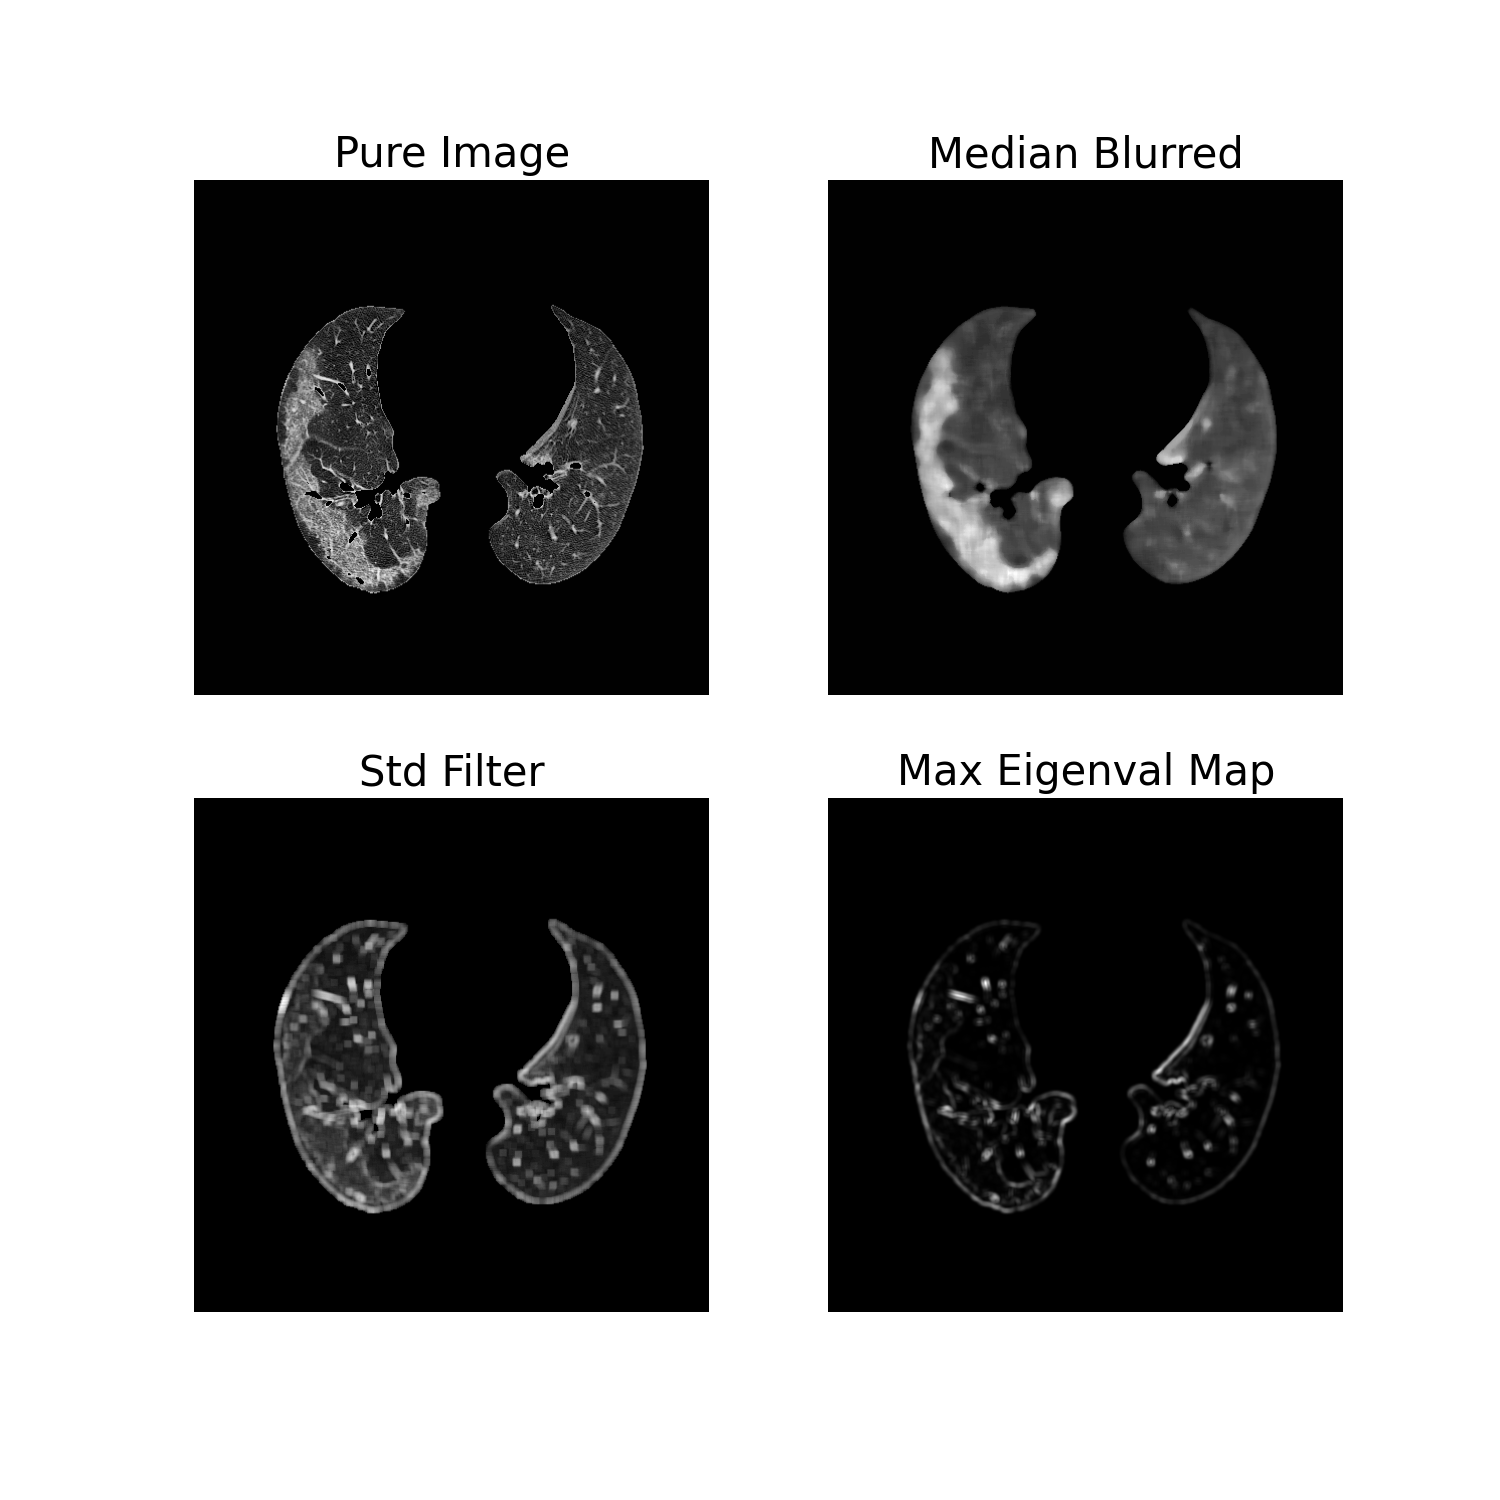
\includegraphics[scale=.33]{./img/Multi_Channel.png}
				\vspace{.2cm}			
			\end{column}
			\begin{column}{.3\textwidth}
				\begin{block}{Single Voxel}
					\begin{itemize}\setlength\itemsep{0.5em}
						\item Histogram Equalized 
						\item Gamma Corrected ($\gamma = 1.5$)
					\end{itemize}			
				\end{block}
%				\textbf{Single Voxel}:
%				\vspace{.3cm}
				\begin{block}{Neighbouring Voxels}
					\begin{itemize}\setlength\itemsep{0.5em}
						\item Median Blurred ($kernel\, size = 11$)
						\item Standard Deviation Map ($kernel\, size = 3$)						
					\end{itemize}
				\end{block}
				%\begin{itemize}\setlength\itemsep{0.5em}
					
				%	\item Histogram Equlization : 
						
					
				%	\item Gamma Corrected : 
						
					
			%	\end{itemize}			
				%\vspace{.5cm}
				%\textbf{Neighbouring Voxels}:
			%	\vspace{.3cm}
				%\begin{itemize}\setlength\itemsep{0.5em}
					
				%	\item Median Blurred
				%	
				%	\item Standard Deviation Map
				%	
				%\end{itemize}
			\end{column}		
		\end{columns}
		
	\end{frame}
\end{document}